\subsection{Quantitative Evaluation}\label{sec:quality}
In this part, we quantitatively evaluate our proposals on the \pt{} and \sz{} trajectory datasets from two aspects:
(i) visual quality at different zoom levels
and (ii) running time under different sampling rates.

\begin{figure}
 \centering
 \small
 \begin{tabular}{cc}
   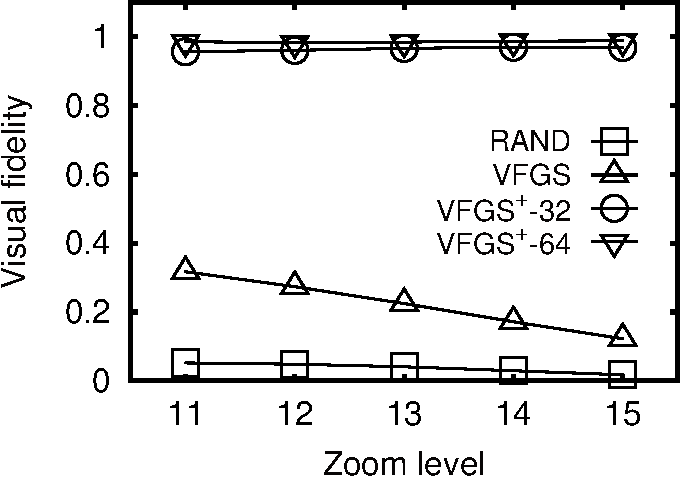
\includegraphics[width=0.44\columnwidth]{pictures/fporto}
   &
   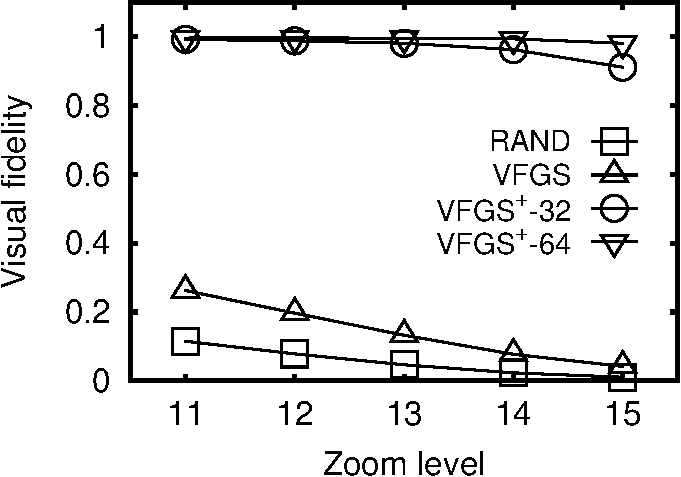
\includegraphics[width=0.44\columnwidth]{pictures/fshenzhen}
   \\
   (A) \pt{}
   &
   (B) \sz{}
 \end{tabular}
 \vspace{-3mm}
 \caption{Visual quality vs. zoom levels.}
 \label{fig:quality}
 \vspace{-3mm}
\end{figure}

\stitle{Visual quality evaluation} We report the \textit{visual quality} of different visualization methods in Figure~\ref{fig:quality}. Visual quality is defined as the $1-loss$, in which $loss$ is the quality loss function in Equation~\eqref{eqref:loss}. The sampling rate is $\alpha=0.5\%$ and the visualization using the full dataset is used as the ground-truth. The results show that $\rand$ always has the lowest  visual quality. $\vats$ has better visual quality than $\rand$ but is significantly outperformed by $\avats$. With $\delta=32$ and $\delta=64$, the minimum visual quality values of $\avats$ are 0.95 and 0.91 for \pt{} and \sz{}, respectively. Moreover, the quality of all methods increases when the zoom level drops, which in line with Theorem~\ref{the:level}.


%We first evaluate the visual fidelity of our proposed methods.
%We measure the visual fidelity of different approaches over the $\full$ by using the $loss()$ function defined in Section~\ref{sec:def}.
%Figure~\ref{fig:fidelity}(A) and (B) show the visual fidelity of $\rand$, $\vats$, $\avats$ with $\delta=32$ and $\avats$ with $\delta=64$ from zoom level 11 to 15 (i.e., overview to detail view) in
%\pt{} and \sz{}, respectively.
%Results show that $\rand$ does not guarantee the visual fidelity of the result.
%Although $\vats$ offers theoretical visual fidelity guarantee w.r.t. the optimal sampled result set with a given sampling rate, it still has room for improvement over the $\full$;
%Moreover, $\avats$ with $\delta=32$ and $\delta=64$ has excellent visual fidelity w.r.t. the $\full$ dataset. The minimum visual fidelity value is 0.95 and 0.91 in \pt{} and \sz{}, respectively.
%It also confirms the superiority of our proposal.
%The visual fidelity of $\avats$ falls with the rising of zoom levels, e.g., from zoom level 11 to 15.
%The reason is the higher zoom level, the more details are expected.


\begin{figure}
 \centering
 \small
 \begin{tabular}{cc}
   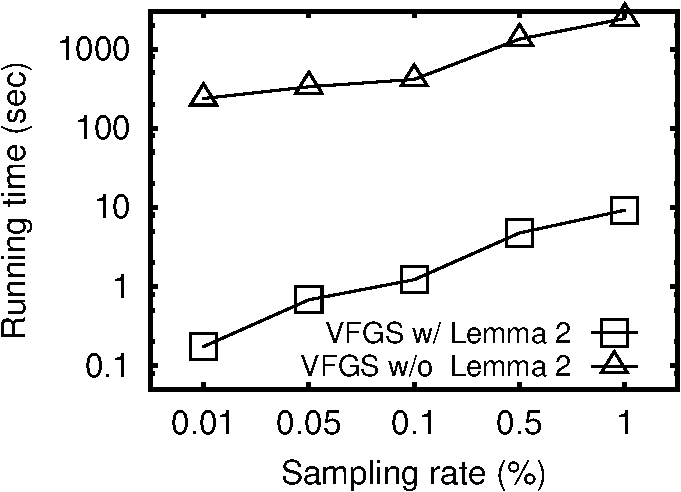
\includegraphics[width=0.44\columnwidth]{pictures/tporto}
   &
   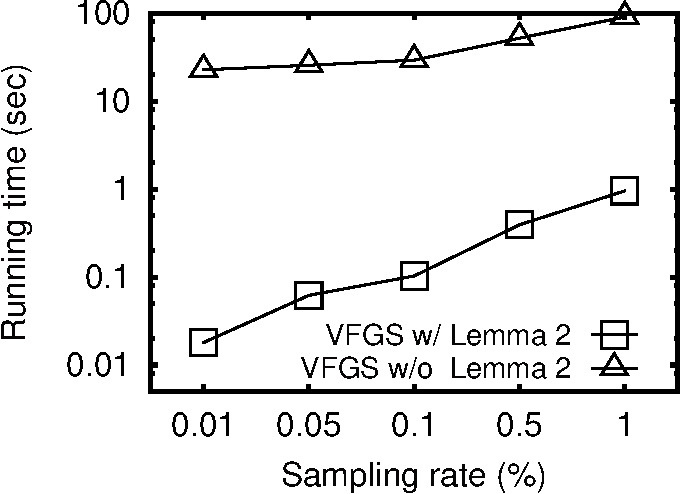
\includegraphics[width=0.44\columnwidth]{pictures/tshenzhen}
   \\
   (A) \pt{}
   &
   (B) \sz{}	
 \end{tabular}
 \vspace{-3mm}
 \caption{Running time of $\vats$ w/ and w/o Lemma~\ref{lem:submodular}.}
 \label{fig:cost}
 \vspace{-3mm}
\end{figure}


\stitle{Running time evaluation}
%\REPORT{
We first conduct an experiment to evaluate the rendering cost by datasize. We vary the number of trajectories from 1000 to 1 million, which are randomly selected from \pt{} dataset. The experimental results are summarized in Table~\ref{tab:gpu}. We observe that the rendering cost is linear with the input data trajectories.
%}
Then, we report the running time of our $\vats$ algorithm in Figure~\ref{fig:cost} by varying the sampling rate from $0.01\%$ to $1\%$. The results show that $\vats$ is quite slow without the submodularity of contribution value, which agrees with Lemma~\ref{lem:submodular} in Section~\ref{sec:opt}.
The optimized $\vats$ (e.g., $\vats$ with Lemma~\ref{lem:submodular}) outperforms $\vats$ by one to three orders of magnitudes on both datasets. The result show that running time of our $\vats$ algorithm is below 1 second in most cases. We have shown that $\vats$ provides good visualization performance with a low sampling rate (e.g., $0.1\%$ or $1\%$) in Section 6.1 and 6.2,  and Table~\ref{tab:gpu} suggests that the rendering latency scales almost linearly with dataset cardinality. By significantly reducing the dataset cardinality with sampling, $\vats$ can effectively reduces the rendering latency to make interactive visualization possible without sacrificing visual quality. For example, rendering the full $\pt{}$ dataset takes about 34 seconds, with a sampling rate of $1\%$, $\vats$ can bring down the rendering latency to less than 1 second.

\begin{table}
	\centering
	\small
	\caption{Visualization rendering cost}
	\begin{tabular}{|c|c|c|} \hline
		No. of trajectories & No. of GPS points & Rendering time (s) \\ \hline
		1,000& 32,648 & 0.016\\ \hline
		10,000& 331,583 & 0.143\\ \hline
		100,000& 3,262,278 & 1.416\\ \hline
		1,000,000& 32,660,845 & 13.950\\ \hline
	\end{tabular}	\label{tab:gpu}
\end{table}
